\begin{center}
	\Huge \textbf{Собственно, матстат...}
\end{center}
\section{Функції від випадкових величин (векторів)}
Для дискретної випадкової величини $\xi$: $\eta = \phi (\xi) \Rightarrow \eta$ - ДВВ. \\
Припустимо, що $\varphi$ - неперервно диференційована. $\xi$ - асолютно неперервна зі щільністю $f_{\xi}(x)$. Розглядаємо $ \eta = \varphi(\xi) $:

\begin{boxteo}
    Нехай $\varphi$ - взаємно-однозначна (бієкція на області значень), та її обернена $\psi$ є неперервно диференційована. (Дифеоморфізм). Тоді:
    $$
    f_{\eta} (y) = \begin{cases}
    \left| \psi '(y) \right| \cdot  f_{\xi }(\psi (y)), & y \in E_{\varphi}\\
        0 & y \notin E_{\varphi}
    \end{cases} = f_{\xi} (\psi (y)) \cdot \left| \psi'(y) \right| \cdot \mathbb{I}_{E_{\varphi}}(y)
    $$
\end{boxteo}

\begin{proof}
Розглядаемо множину B.
$$  \int\limits_{B }^{ }{ f_{\eta} (y)dy} = \mathbb{P} \left\lbrace \eta \in B \right\rbrace =
\mathbb{P} \left\lbrace \varphi(\xi) \in B \right\rbrace = \mathbb{P} \left\lbrace \xi \in \phi^{-1} (B) \right\rbrace =  \int\limits_{\phi^{-1} (B)}^{}{f_{\xi}(x)dx} =
$$

$$
= \left| \begin{gathered}
  \varphi(x) = y \\
  x = \psi(y) \\
  J = \psi'(y) = J_{\psi}
\end{gathered} \right|  =  \int\limits_{B \cap E_{\varphi}}^{ }{ f_{\xi} (\psi (y)) \cdot \left| J_{\psi} (y)  \right| dy} =  \int\limits_{B}^{ }{f_{\xi} (\psi (y)) \cdot \left| \psi'(y) \right| \cdot \mathbb{I}_{E_{\varphi}}(y)dy}
$$
\end{proof}
\begin{boxteo}
Нехай $\phi$ не є ін'єкцією, але ''розпадається'' на декілька таких.
$$
\begin{gathered}
 \varphi_1 (x) = x^2, x\in (- \i, 0)\\
 \varphi_2(x) = x^2, x \in [0, +\i]\\
 E_{\varphi_1} = (0, + \i) \quad E_{\varphi_2} = (0, + \i)\\
 \psi (x) = y   \quad x^2 = y  \quad x = \pm \sqrt{y} \\
 \psi_1(y) = - \sqrt{y} \quad \psi_2(y) = \sqrt{y}
\end{gathered} \qquad \quad
\begin{gathered}
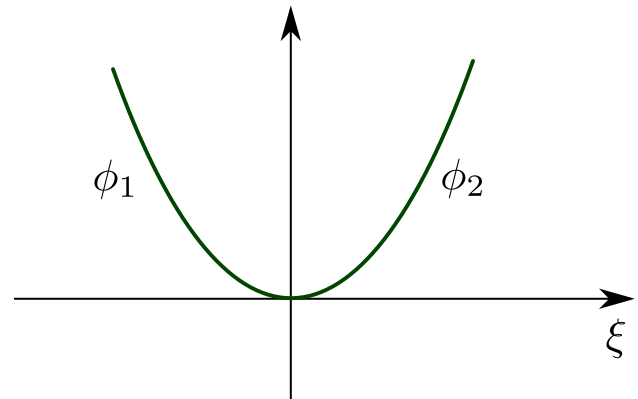
\includegraphics[scale=0.24]{assets/lectures_part_3-7a9fde69.png}
\end{gathered}
$$
\textbf{Тоді: } \fbox{$ f_{\eta} (y) =  \sum\limits_{i = 1}^{ n}{ f_{\xi} (\psi_i (y)) \cdot \left| \psi_i'(y) \right| \cdot \mathbb{I}_{E_{\varphi_i}}(y)}$}.
\end{boxteo}
\begin{proof}
  Розглядаемо множину B.
  $$  \int\limits_{B }^{ }{ f_{\eta} (y)dy} = \mathbb{P} \left\lbrace \eta \in B \right\rbrace =
 \mathbb{P} \left\lbrace \xi \in \phi_1^{-1} (B) \cup \cdots \cup \xi \in \phi_n^{-1} (B) \right\rbrace =
  $$
  $$
  =  \sum\limits_{i = 1}^{n}{ \mathbb{P} \left\lbrace \xi \in \phi_i^{-1} (B) \right\rbrace  }  - \text{ надалі доведення зводиться до попередньої теореми.}
  $$
  \end{proof}

 \subsection{Функції від випадкових векторів.}
 Розглядаємо $ \overline{\xi} = \begin{bmatrix}
  \xi_1 \\
  \xi_2
 \end{bmatrix} \quad \eta = \varphi(\xi_1, \xi_2)$.\\
 1. Для дискретного випадку обчислення тривіальні.\\
 2. $ \overline{\xi} $ - абсолютно неперервний випадковий вектор.
 $$ f_{\overline{\xi}} (\overline{x}) \Rightarrow \eta = \varphi( \overline{\xi}) \quad f_{\eta} (y)=? \quad \varphi: \mathbb{R}^n \to \mathbb{R}$$
\begin{boxteo}
    $ \varphi: \mathbb{R}^n \to \mathbb{R}^n. \varphi$ - взаємно-однозначна $ \Rightarrow \psi = \varphi^{-1}$.\\
    $\varphi, \psi $ - дифеоморфізми $ \Rightarrow  \exists J_{\psi} ( \overline{y}) $ - якобіан. Тоді:
    $$
    f_{\overline{\eta}}  (\overline{y}) = f_{\overline{\xi}} (\psi(\overline{y})) \cdot \left| J_{\psi (\overline{y})} \right| \cdot   \mathbb{I}_{E_{\varphi}} (\overline{y})
    $$
\end{boxteo}
\begin{boxteo}
    $\varphi$ розпадаэться на суму ін'єктивних функцій  $\varphi_1, ..., \varphi_k$.\\
    $ \varphi^{-1}_i = \psi_i. \quad E_i$ - область значень $ \varphi_i. \quad J_{\psi_i}$ - якобіан $ \psi_i$. Тоді:
    $$
    f_{\eta} (\overline{y}) =  \sum\limits_{i = 1}^{ k}{ f_{\overline{\xi}} ( \psi_i( \overline{y})) \cdot \left| J_{\varphi_i } (\overline{y}) \right|  \cdot \mathbb{I}_{E_{\varphi_i}} (\overline{y})}
    $$
\end{boxteo}
Часто будемо використовувати: \fbox{$f_{\xi_1 + \xi_2} (y) =  \int\limits_{-\infty}^{ +\infty}{ f_{\overline{\xi} } (x, y-x) dx}$}.\\
Якщо $ \xi_1 \independent \xi_2: $ \fbox{$ f_{\xi_1 + \xi_2} (y) =  \int\limits_{-\infty}^{ +\infty}{ f_{\xi_1} (x) \cdot f_{\xi_2} (y-x) dx}$}.\\ Також: $f_{\xi_1 + \xi_2} (y) = (f_{\xi_1} \circledast f_{\xi2} (y))$ - згортка.
\subsection{Загальний алгоритм знаходження щільності функції від випадкових векторів.}
Розглядаємо $ \eta = \varphi( \overline{\xi}) \quad f_{\eta} (z) = ?$.
$$
F_{\eta} = \mathbb{P} \left\lbrace  \eta < z \right\rbrace = \mathbb{P} \left\lbrace \varphi(\xi_1, \xi_2) < z \right\rbrace = \left| \left\lbrace (x,y) \in \mathbb{R} \bigg| \varphi(x,y) < z \right\rbrace = D_z \right|  =
$$
$$
 =  \iint\limits_{D_z}^{}{f_{\overline{\xi} (x,y ) dxdy}} \Longrightarrow f_\eta (z)  = F_\eta' (z)
$$
Знайдемо щільності розподілу суми, добутку та частки випадкових величин.
$$\xi_1, \xi_2, f_{\overline{\xi} }(x,y) \Longrightarrow f_{\xi_1 + \xi_2} (z), f_{\xi_1 \cdot \xi_2} (x,y), f_{\xi_1/ \xi_2} (x,y) - ?$$
\textbf{Сума:} $ F_{\xi_1 + \xi_2} (z) = \mathbb{P} \left\lbrace \xi_1 + \xi_2 < z \right\rbrace = \mathbb{P} \left\lbrace \overline{\xi} \in D_z \right\rbrace =
  \iint\limits_{D_z}^{ }{ f_{\overline{\xi}} ( x,y) dxdy} =
$
$$
\begin{gathered}
=  \int\limits_{-\infty}^{ +\infty}{ dx  \int\limits_{-\infty}^{ z-x}{f_{\overline{\xi}}(x,y)dy}}\\
 f_{\xi_1 + \xi_2} (z) = \int\limits_{-\infty}^{ +\infty}{ f_{\overline{\xi}} (x, z-x) dx}
\end{gathered}\qquad \quad
\begin{gathered}
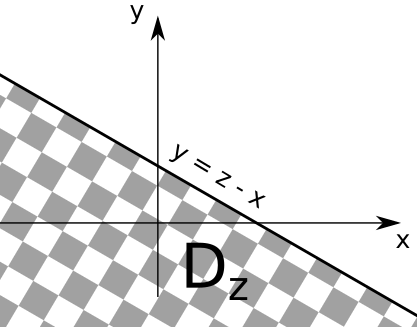
\includegraphics[scale=0.45]{assets/lectures_part_3-43a27a3a.png}
\end{gathered}
$$
$$
f_{\xi_1 + \xi_2} (z) =  \int\limits_{-\infty}^{ +\infty}{ f_{\overline{\xi}}(x, z-x)dx = \left| \xi_1 \independent \xi_2 \right| =  \int\limits_{-\infty}^{ +\infty}{ f_{\xi_1} (x) \cdot f_{\xi_2} (z-x) dx }}
$$
\textbf{Добуток: } Шукаємо $ f_{\xi_1 \cdot \xi_2 } \quad F_{\xi_1 \cdot \xi_2}= \mathbb{P} \left\lbrace \xi_1 \cdot \xi_2 < z \right\rbrace$.\\
$$
\begin{gathered}
x * y < z \Leftrightarrow \left[ \begin{gathered}
\begin{cases}
    y < \frac{z}{x}\\
    x> 0
\end{cases}\\
\begin{cases}
    y > \frac{z}{x}\\
    x < 0
\end{cases}
\end{gathered}
 \right.
\end{gathered}
 \qquad
 \begin{gathered}
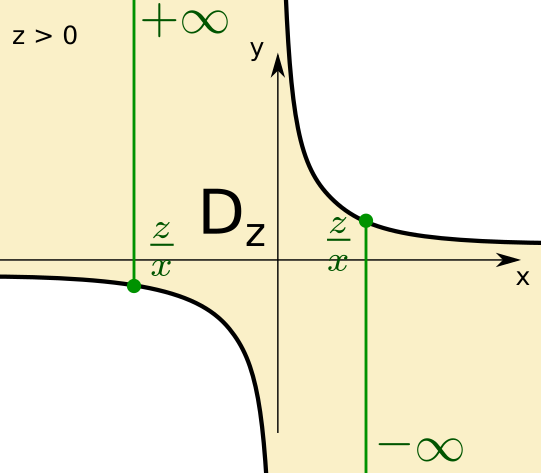
\includegraphics[scale=0.4]{assets/lectures_part_3-5c275c57.png}
 \end{gathered}
$$
$$
F_{\xi_1 \cdot \xi_2} (z) =  \iint\limits_{D_z}^{ }{ f_{\overline{\xi}} (x,y) dxdy} =  \int\limits_{-\infty}^{0}{dx  \int\limits_{ \frac{z}{x}  }^{ +\infty}{ f_{\overline{\xi}} (x,y )dy}} +  \int\limits_{0}^{ +\infty}{ dx  \int\limits_{-\infty}^{ \frac{z}{x} }{f_{\overline{\xi}} (x,y )dy}}
$$
$$
f_{\xi_1 \cdot \xi_2} (z) = -  \int\limits_{-\infty}^{ 0}{ f_{\overline{\xi}}(x, \frac{z}{x})\cdot \frac{1}{x} dx  } + \int\limits_{0}^{ + \infty}{ f_{\overline{\xi}}(x, \frac{z}{x})\cdot \frac{1}{x} dx  }
$$
